\chapter{Mérési eredmények} \label{resultsChapter}

A méréseket a következő paraméterekkel rendelkező számítógépen végeztem:
\begin{itemize}
	\item	CPU: 11th Gen Intel(R) Core(TM) i5-11300H @ 3.10GHz
	\item	GPU: NVIDIA GeForce RTX 3050Ti 
	\item	RAM: 24 GB DDR4 
	\item	OS: Windows 10 Education 22H2 
	\item	Compiler: NVCC V12.0.140
	
\end{itemize}

\section{A mérések menete}
Az algoritmusokhoz külön CPU és GPU kódot készítettem. Az eljárás érdemi részét megszakítás nélkül GPU-n végeztem, míg CPU-n a kezdeti értékeket állítottam be, különböző diagnosztikai kiíratásokat végeztem, illetve a parancssori argumentumok feldolgozását kezeltem. A futásidők méréséhez az NVIDIA által készített Nsight Compute(R) programot használtam, mely több szempontból képes CUDA kerneleket elemezni: futási idő, memória kihasználtsága, grid mérete, blokk mérete, szálanként regiszterek száma és még tovább. A program futását \ref{fig:nsight-compute}. ábrán ábrázoltam. 

\begin{figure}[ht!]
	\centering
	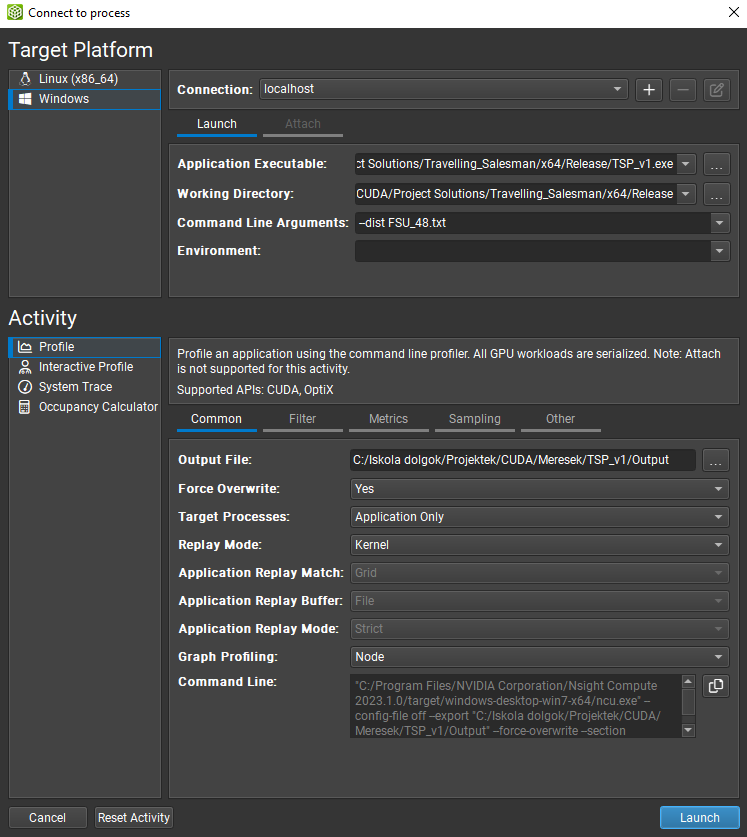
\includegraphics[width=85mm, keepaspectratio]{figures/nsight-compute-config.png}
	\caption{Az NVIDIA Nsight Compute programban egy mérés összeállításához be kell állítani a mérendő exe fájlt, a munkamappát, illetve a szükséges parancssori argumentumokat}
	\label{fig:nsight-compute-config}
\end{figure}

\begin{figure}[ht!]
	\centering
	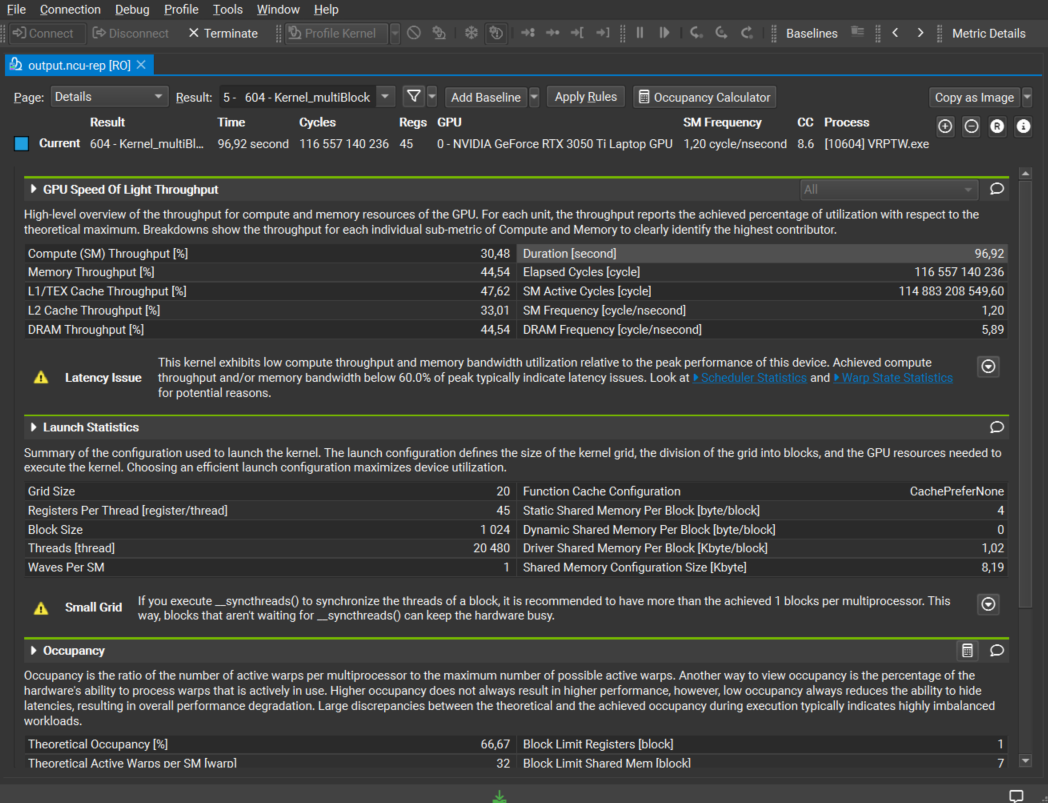
\includegraphics[width=125mm, keepaspectratio]{figures/nsight-compute2.png}
	\caption{Az NVIDIA Nsight Compute program adatok széles tárházával látja el a programozót }
	\label{fig:nsight-compute}
\end{figure}




Számomra a legfontosabb a futásidő volt, ezt több különböző bemenetre és konfigurációra lemértem, majd táblázatosan összegyűjtöttem.

\section{Mérési eredmények}

A továbbiakban táblázatokba szedtem az egyes algoritmusokon végzett profilozó méréseim eredményeit. A futásidők időegysége másodperc, mert ilyen nagyságrendben mozogtak az értékek. Többször lefuttattam a programokat ugyanolyan paraméterek mellett, ebből lejegyeztem az átlagos eredményeket (10 futás számtani közepe) és a legkisebb kapott megoldást. Amikor nem optimális egy mérési eredmény, akkor százalékos arányban melléírtam, hogy mennyivel magasabb az elméleti minimumnál.

A CVRPTW mérése során tapasztaltam először olyat, hogy néha a program egyáltalán nem talált megoldást. Ott új oszlopot vettem fel "Hiba (\%)" névvel. Azt mutatja, hogy a programfuttatások hány százalékában nem sikerült egyáltalán megoldást találni. Ilyenkor az átlagolást a sikeres futtatásokból számoltam.

\newpage

\section{TSP első verzió}

Teszteléshez szükségem volt ismert eredményű adathalmazokra. A Floridai Állami Egyetem weboldalán \cite{TSPdataset} elérhető bárki számára több adathalmaz, különböző adatstruktúrában. Számomra a [fájlnév]\_d.txt nevű fájlok voltak hasznosak, ugyanis abban megtalálhatóak a szomszédossági mátrix költségei táblázatos alakban. Az itt található 6 adathalmazon végigfuttattam az algoritmusomat több konfigurációban. Mindig 10-szer ismételtem meg a futást, és lejegyeztem az eredmények átlagát (számtani középpel), illetve minimumát. Nagy adathalmaz esetén hosszú a futásidő profilozó módban, ezért időmérés céljából egyszer futtattam újra ugyanazon beállításokkal. A TSP első verziójában a feromonmátrix és az élsúlyok tárolása csak \textit{double} formátumban történik. Az összehasonlíthatóság érdekében egy iteráció során 20 random, és 500 tudatos hangya fut. A kezdeti feromon érték 1000, az elnyomási tényező \( \rho = 0.75 \), a jutalmazási arány 100, amely csak a 2. iterációtól érvényes (ha van). 

Az egyes mérések eredményei a \ref{table:TSPv1_5} - \ref{table:TSPv1_48}. táblázatokból olvashatóak.

% Size = 5
\begin{table}[ht!]
	\centering
	\begin{tabular}{|p{2cm}||p{3cm}|p{3.5cm}|p{3.5cm}|}
		\hline
		\multicolumn{4}{|c|}{FIVE : 5 csúcs, minimális út : 19, átlagos út : 24} \\
		\hline
		& Futásidő (ms) & Végeredmény átlag & Végeredmény min.\\
		\hline
		\textbf{1 rep} & & &\\
		32 ant& 7,84 & 20,2 (+6,3\%) & 19\\
		256 ant & 19,1 & 20,8 (+9,5\%) & 19\\
		1024 ant & 76,1 & 20,8 (+9,5\%) &	19\\
		\hline
		\textbf{10 rep} & & &\\
		256 ant & 137,3 & 19 &	19\\
		1024 ant & 424 &	19 &	19\\
		\hline
	\end{tabular}
	\caption{Elsőnek egy kicsi, a kezdőponton kívül 4 állomásból álló gráfon próbáltam ki az algoritmust.}
	\label{table:TSPv1_5}
\end{table}

% Size = 15
\begin{table}[ht!]
	\centering
	\begin{tabular}{|p{2cm}||p{3cm}|p{3.5cm}|p{3.5cm}|}
		\hline
		\multicolumn{4}{|c|}{P01 : 15 csúcs, minimális út : 291, átlagos út : 662} \\
		\hline
		& Futásidő (s) & Végeredmény átlag & Végeredmény min.\\
		\hline
		\textbf{1 rep} & & &\\
		1024 ant & 0,925 & 370,2 (+27,2\%) & 291 \\
		2048 ant & 1,18 & 365 (+25,4\%) & 327 (+12,4\%) \\
		4096 ant & 1,20 & 359,7 (+23,6\%) & 332 (+14,1\%)\\
		\hline
		\textbf{10 rep} & & &\\
		1024 ant & 11,39 & 350,4 (+20,4\%) & 291\\
		2048 ant & 11,47 & 328 (+12,5\%) & 295 (+1,4\%)\\
		4096 ant & 11,59 & 336,8 (+15,7\%) & 291\\
		16384 ant & 13,21 & 326,2 (+12,1\%) & 295 (+1,4\%) \\
		20480 ant & 13,46 & 323,4 (+11,1\%) & 291 \\
		\hline
	\end{tabular}
	\caption{15 csúcsú gráfon futtatott TSP v1}
	\label{table:TSPv1_15}
\end{table}

A 17 vagy nála nagyobb gráfok esetében az 1 iterációs algoritmusok már olyan rosszul teljesítettek, hogy a méréseket legalább 10 iterációval folytattam.

% Size = 17
\begin{table}[ht!]
	\centering
	\begin{tabular}{|p{2cm}||p{3cm}|p{3.5cm}|p{3.5cm}|}
		\hline
		\multicolumn{4}{|c|}{GR : 17 csúcs, minimális út : 2085} \\
		\hline
		& Futásidő (s) & Végeredmény átlag & Végeredmény min.\\
		\hline
		\textbf{10 rep} & & & \\
		1024 ant & 14,85 & 2391,3 (+14,7\%) & 2151 (+3,2\%)\\
		2048 ant & 14,88 & 2363,4 (+13,5\%) & 2085\\
		4096 ant & 14,97 & 2279,6 (+9,3\%) & 2097 (+0,6\%) \\
		8192 ant & 15,15 & 2306,4 (+10,6\%) & 2207 (+5,9\%)\\
		16384 ant & 15,49 & 2250,5 (+7,9\%) & 2085 \\
		20480 ant & 15,68 & 2221,7 (+6,6\%) & 2085 \\
		\hline
	\end{tabular}
	\caption{17 csúcsú gráfon futtatott TSP v1}
	\label{table:TSPv1_17}
\end{table}

% Size = 26
\begin{table}[ht!]
	\centering
	\begin{tabular}{|p{2cm}||p{3cm}|p{3.5cm}|p{3.5cm}|}
		\hline
		\multicolumn{4}{|c|}{FRI26 : 26 csúcs, minimális út : 937, átlagos út : 2693} \\
		\hline
		& Futásidő (s) & Végeredmény átlag & Végeredmény min.\\
		\hline
		\textbf{10 rep} & & & \\
		1024 ant & 39,72 & 1386,1 (+47,9\%) & 1249 (+33,3\%)\\
		2048 ant & 39,73 & 1367,1 (+45,9\%) & 1221 (+30,3\%) \\
		4096 ant & 39,82 & 1227,6 (+31\%) & 1121 (+19,6\%) \\
		8192 ant & 40,14 & 1158,7 (+23,7\%) & 1102 (+17,6\%) \\
		16384 ant & 40,70 & 1132,1 (+20,8\%) & 1075 (+14,7\%) \\
		20480 ant & 42,72 & 1152,3 (+23\%) & 1097 (+17,1\%) \\
		\hline
	\end{tabular}
	\caption{26 csúcsú gráfon futtatott TSP v1}
	\label{table:TSPv1_26}
\end{table}

% Size = 42
\begin{table}[ht!]
	\centering
	\begin{tabular}{|p{2cm}||p{3cm}|p{3.5cm}|p{3.5cm}|}
		\hline
		\multicolumn{4}{|c|}{DANTZIG42 : 42 csúcs, minimális út : 699, átlagos út : 3110,5} \\
		\hline
		& Futásidő (s) & Végeredmény átlag & Végeredmény min.\\
		\hline
		\textbf{10 rep} & & & \\
		1024 ant & 115,41 & 1735,7 (+148\%) & 1554 (+122\%) \\
		2048 ant & 113,94 & 1420 (+103\%) & 1252 (+79\%) \\
		16384 ant & 114,34 & 987,7 (+41\%) & 906 (+30\%) \\
		20480 ant & 113,55 & 931,6 (+33\%) & 879 (+26\%) \\
		\hline
	\end{tabular}
	\caption{42 csúcsú gráfon futtatott TSP v1}
	\label{table:TSPv1_42}
\end{table}

% Size = 48
\begin{table}[htbp!]
	\centering
	\begin{tabular}{|p{2cm}||p{3cm}|p{3.5cm}|p{3.5cm}|}
		\hline
		\multicolumn{4}{|c|}{ATT48 : 48 csúcs, minimális út : 33523, átlagos út : 157686,9} \\
		\hline
		& Futásidő (s) & Végeredmény átlag & Végeredmény min.\\
		\hline
		\textbf{10 rep} & & & \\
		1024 ant & 156,7 & 79993,2 (+139\%) & 75601 (+126\%) \\
		8192 ant & 152,82 & 56097,9 (+67\%) & 51139 (+53\%) \\
		16384 ant & 153,78 & 50197,2 (+50\%) & 47387 (+41\%) \\
		20480 ant & 154,28 & 46360,8 (+38,3\%) & 43167 (+28,77\%) \\
		\hline
	\end{tabular}
	\caption{48 csúcsú gráfon futtatott TSP v1}
	\label{table:TSPv1_48}
\end{table}

\newpage
\newpage

\section{TSP második (konzisztens) verzió}
Azért, hogy az előző fejezetben látott első verzióval érdemben össze tudjam hasonlítani a mostani verziót, hasonló iterációs számokat választottam: 1 rep-en belül 20 random hangyát követ 500 tudatos hangya. Az adathalmaz is az előbbi \cite{TSPdataset} helyről származó csomag. A számértékeket összevetve szembetűnő a gyorsulás az előző verzióhoz képest. A legfőbb szerepe ebben úgy gondolom, hogy az adattípus \textit{double}-ről \textit{float}-ra cserélése, illetve a függvények között szigorú pointer alapú paraméterátadás jelentette.

Az egyes mérések eredményei a \ref{table:TSPv2_15} - \ref{table:TSPv2_48}. táblázatokból olvashatóak ki.

% Size = 15
\begin{table}[ht!]
	\centering
	\begin{tabular}{|p{2cm}||p{3cm}|p{3.5cm}|p{3.5cm}|}
		\hline
		\multicolumn{4}{|c|}{P01 : 15 csúcs, minimális út : 291, átlagos út : 662} \\
		\hline
		& Futásidő (s) & Végeredmény átlag & Végeredmény min.\\
		\hline
		\textbf{10 rep} & & &\\
		1024 ant & 2,69 & 320,0 (+10\%) & 307 (+5,5\%) \\
		2048 ant & 2,82 & 307,6 (+5,7\%) & 291\\
		4096 ant & 2,97 & 305,4 (+4,9\%) & 291\\
		8192 ant & 3,19 & 300,2 (+3,2\%) & 291\\
		12288 ant & 3,50 & 296,4 (+1,9\%) & 291\\
		16384 ant & 3,73 & 294,6 (+1,2\%) & 291\\
		20480 ant & 3,92 & 295,4 (+1,5\%) & 291\\
		\hline
		\textbf{30 rep} & & &\\
		1024 ant & 8,05 & 301,6 (+3,6\%) & 291\\
		20480 ant & 13,37 & 291 & 291\\
		\hline
	\end{tabular}
	\caption{15 csúcsú gráfon futtatott TSP v2}
	\label{table:TSPv2_15}
\end{table}

% Size = 17
\begin{table}[ht!]
	\centering
	\begin{tabular}{|p{2cm}||p{3cm}|p{3.5cm}|p{3.5cm}|}
		\hline
		\multicolumn{4}{|c|}{GR : 17 csúcs, minimális út : 2085} \\
		\hline
		& Futásidő (s) & Végeredmény átlag & Végeredmény min.\\
		\hline
		\textbf{10 rep} & & & \\
		1024 ant & 3,54 & 2246 (+7,7\%) & 2094 (+0,4\%)\\
		2048 ant & 3,69 & 2237,7 (+7,3\%) & 2207 (+5,9\%)\\
		4096 ant & 3,69 & 2196,5 (+5,3\%) & 2142 (+2,7\%)\\
		8192 ant & 3,89 & 2211,5 (+6,1\%) & 2170 (+4,1\%)\\
		16384 ant & 4,37 & 2179,2 (+4,5\%) & 2129 (+2,1\%)\\
		20480 ant & 4,55 & 2175,1 (+4,3\%) & 2134 (+2,4\%) \\
		\hline
		\textbf{30 rep} & & & \\
		20480 ant & 13,38 & 2146,5 (+3\%) & 2103 (+0,9\%) \\
		\hline
	\end{tabular}
	\caption{17 csúcsú gráfon futtatott TSP v2}
	\label{table:TSPv2_17}
\end{table}

% Size = 26
\begin{table}[ht!]
	\centering
	\begin{tabular}{|p{2cm}||p{3cm}|p{3.5cm}|p{3.5cm}|}
		\hline
		\multicolumn{4}{|c|}{FRI26 : 26 csúcs, minimális út : 937, átlagos út : 2693} \\
		\hline
		& Futásidő (s) & Végeredmény átlag & Végeredmény min.\\
		\hline
		\textbf{10 rep} & & & \\
		1024 ant & 9,00 & 1393 (+48,7\%) & 1347 (+43,8\%)\\
		2048 ant & 9,23 & 1363,1 (+45,5\%) & 1288 (+37,5\%)\\
		4096 ant & 9,43 & 1215,3 (+29,7\%)& 1163 (+24,1\%)\\
		8192 ant & 9,72 & 1136,9 (+21,3\%) & 1055 (+12,6\%)\\
		16384 ant & 10,82 & 1104,9 (+17,8\%) & 1007 (+7,5\%) \\
		20480 ant & 11,61 & 1111,7 (+18,6\%) & 1058 (+12,9\%) \\
		\hline
		\textbf{30 rep} & & & \\
		20480 ant & 32,93 & 1098,2 (+17,2\%) & 1047 (+11,7\%) \\
		\hline
	\end{tabular}
	\caption{26 csúcsú gráfon futtatott TSP v2}
	\label{table:TSPv2_26}
\end{table}

% Size = 42
\begin{table}[ht!]
	\centering
	\begin{tabular}{|p{2cm}||p{3cm}|p{3.5cm}|p{3.5cm}|}
		\hline
		\multicolumn{4}{|c|}{DANTZIG42 : 42 csúcs, minimális út : 699, átlagos út : 3110,5} \\
		\hline
		& Futásidő (s) & Végeredmény átlag & Végeredmény min.\\
		\hline
		\textbf{10 rep} & & & \\
		1024 ant & 26,19 & 1601,3 (+129\%) & 1018 (+46\%)\\
		2048 ant & 26,61 & 1488,4 (+113\%) & 1319 (+89\%) \\
		4096 ant & 27,02 & 1286,7 (+84\%) & 1168 (+67\%)\\
		8192 ant & 27,57 & 1118,3 (+60\%) & 1004 (+44\%) \\
		16384 ant & 31,2 & 1014,7 (+45\%) & 909 (+30\%)\\
		20480 ant & 33,31 & 964,9 (+38\%) & 822 (+17,6\%) \\
		\hline
		\textbf{30 rep} & & & \\
		20480 ant & 99,83 & 972,8 (+39,2\%) & 886 (+26,75\%) \\
		\hline
	\end{tabular}
	\caption{42 csúcsú gráfon futtatott TSP v2}
	\label{table:TSPv2_42}
\end{table}

% Size = 48
\begin{table}[htbp!]
	\centering
	\begin{tabular}{|p{2cm}||p{3cm}|p{3.5cm}|p{3.5cm}|}
		\hline
		\multicolumn{4}{|c|}{ATT48 : 48 csúcs, minimális út : 33523, átlagos út : 157686,9} \\
		\hline
		& Futásidő (s) & Végeredmény átlag & Végeredmény min.\\
		\hline
		\textbf{10 rep} & & & \\
		1024 ant & 38,12 & 84660,7 (+153\%) & 67541 (+102\%) \\
		2048 ant & 38,63 & 72522,8 (+116\%) & 64969 (+94\%) \\
		4096 ant & 39,14 & 62808,6 (+87\%) & 53395 (+59\%) \\
		8192 ant & 39,69 & 59604,8 (+78\%) & 52514 (+57\%) \\
		16384 ant & 41,56 & 48618,2 (+45\%) & 46227 (+38\%)\\
		20480 ant & 41,93 & 49879,9 (+48,8\%) & 45836 (+36,7\%)\\
		\hline
		\textbf{30 rep} & & & \\
		20480 ant & 124,72 & 47562,9 (+41,9\%) & 44144 (+31,7\%) \\
		\hline
	\end{tabular}
	\caption{48 csúcsú gráfon futtatott TSP v2}
	\label{table:TSPv2_48}
\end{table}

\newpage

\section{VRP}
A VRP-hez először nem értettem, hogy miért nem találtam külön adathalmazt. Később megértettem, hogy mivel nincs megadva egyéb feltétel, általában teljesen mindegy, hogy hány járművet használhat az algoritmus, a legjobban akkor fog járni, ha az összes állomást ugyanazon járművel járja végig. A VRP-hez is készült külön kódimplementáció. Ez azért jó, mert amikor különböző feltételeket szabunk meg, elég azok figyelembe vételével kiegészíteni a programot.


\section{CVRP}
Az első feltételes útvonaltervezést igénylő algoritmus, amivel foglalkoztam a kapacitásos járműútvonal-tervezés. Adathalmazt a következő helyről szedtem: \cite{CVRPdataset}.
Az iterációk az előzőeknél látottakkal megegyezőek: 1 rep-en belül 20 random hangyát követ 500 tudatos hangya.

Az egyes mérések eredményei a \ref{table:CVRP_gr17} - \ref{table:CVRP_att48}. táblázatokból olvashatóak ki.

% Size = 17
\begin{table}[ht!]
	\centering
	\begin{tabular}{|p{2cm}||p{3cm}|p{3.5cm}|p{3.5cm}|}
		\hline
		\multicolumn{4}{|c|}{17-city problem (Groetschel): 17 csúcs, minimális út: 2685} \\
		\hline
		& Futásidő (s) & Végeredmény átlag & Végeredmény min.\\
		\hline
		\textbf{10 rep} & & & \\
		1024 ant & 2,96 & 3158,7 (+17,6\%) & 2726 (+1,5\%) \\
		16384 ant & 3,44 & 2790,4 (+3,9\%) & 2711 (+1\%) \\
		20480 ant & 3,83 & 2800,5 (+4,3\%) & 2685 \\
		\hline
		\textbf{30 rep} & & & \\
		1024 ant & 6,05 & 2975,2 (+10,8\%) & 2685\\
		16384 ant & 10,64 & 2846,2 (+6\%) & 2727 (+1,5\%) \\
		20480 ant & 13,80 & 2758,5 (+2,7\%) & 2685 \\
		\hline
		\textbf{50 rep} & & & \\
		1024 ant & 9,97 & 2927,5 (+9\%) & 2685 \\
		16384 ant & 17,64 & 2737,25 (+1,9\%) & 2685\\
		20480 ant & 18,51 & 2724,9 (+1,5\%) & 2685\\
		\hline
	\end{tabular}
	\caption{gr17: 17 csúcsú gráfon futtatott CVRP}
	\label{table:CVRP_gr17}
\end{table}

% Size = 21
\begin{table}[ht!]
	\centering
	\begin{tabular}{|p{2cm}||p{3cm}|p{3.5cm}|p{3.5cm}|}
		\hline
		\multicolumn{4}{|c|}{21-city problem (Groetschel): 21 csúcs, minimális út: 3704} \\
		\hline
		& Futásidő (s) & Végeredmény átlag & Végeredmény min.\\
		\hline
		\textbf{10 rep} & & & \\
		1024 ant & 2,96 & 5026,3 (+35,7\%) & 4389 (+18,5\%) \\
		16384 ant & 4,75 & 4217 (+13,9\%) & 4068 (+9,8\%) \\
		20480 ant & 5,72 & 4103,3 (+10,8\%) & 3903 (+5,4\%) \\
		\hline
		\textbf{30 rep} & & & \\
		1024 ant & 8,31 & 4770,5 (+28,8\%) & 4001 (+8\%) \\
		16384 ant & 12,17 & 4105,4 (+10,8\%)& 3864 (+4,3\%) \\
		20480 ant & 16,61 & 4133 (+11,6\%)& 3881 (+4,8\%) \\
		\hline
		\textbf{50 rep} & & & \\
		1024 ant & 19,76 & 4467,5 (+20,6\%)& 3758 (+1,5\%)\\
		16384 ant & 22,73 & 4259,3 (+15\%) & 4090 (+10,4\%)\\
		20480 ant & 28,03 & 4211,6 (+13,7\%)& 4053 (+9,4\%)\\
		\hline
	\end{tabular}
	\caption{gr21: 21 csúcsú gráfon futtatott CVRP}
	\label{table:CVRP_gr21}
\end{table}

% Size = 33
\begin{table}[ht!]
	\centering
	\begin{tabular}{|p{2cm}||p{3cm}|p{3.5cm}|p{3.5cm}|}
		\hline
		\multicolumn{4}{|c|}{Augerat et al: 33 csúcs, minimális út: 742} \\
		\hline
		& Futásidő (s) & Végeredmény átlag & Végeredmény min.\\
		\hline
		\textbf{10 rep} & & &\\
		1024 ant & 5,62 & 1571,62 (+111,8\%) & 1283,05 (+72,9\%)\\
		16384 ant & 8,61 & 1496,24 (+101,6\%) & 1342,16 (+80,7\%) \\
		20480 ant & 13,01 & 1470,99 (+98,3\%) & 1310,18 (+76,6\%) \\
		\hline
		\textbf{30 rep} & & & \\
		1024 ant & 22,74 & 1529,4 (+106\%)& 1351,81 (+82\%)\\
		16384 ant & 23,68 & 1375,43 (+85,3\%) & 1209,97 (+63\%)\\
		20480 ant & 35,24 & 1415,17 (+90,7\%) & 1182,57 (+59,4\%) \\
		\hline
		\textbf{50 rep} & & & \\
		1024 ant & 24,91 & 1434,34 (+93,9\%) & 1230 (+65,8\%)\\
		16384 ant & 41,26 & 1421,19 (+91,5\%) & 1361,51 (+83,5\%) \\
		20480 ant & 61,01 & 1402,18 (+89\%) & 1092,92 (+47,3\%) \\
		\hline
	\end{tabular}
	\caption{a33: 33 csúcsú gráfon futtatott CVRP}
	\label{table:CVRP_a33}
\end{table}

% Size = 48
\begin{table}[ht!]
	\centering
	\begin{tabular}{|p{2cm}||p{3cm}|p{3.5cm}|p{3.5cm}|}
		\hline
		\multicolumn{4}{|c|}{Rinaldi,Yarrow/Araque: 48 csúcs, minimális út: 40002} \\
		\hline
		& Futásidő (s) & Végeredmény átlag & Végeredmény min.\\
		\hline
		\textbf{10 rep} & & & \\
		1024 ant & 44,28 & 89736,85 (+124\%) & 56813,06 (+42\%) \\
		16384 ant & 44,86 & 83208,23 (+108\%) & 57162,13 (+43\%) \\
		20480 ant & 48,89 & 89271,67 (+123\%) & 56966,07 (+42\%) \\
		\hline
		\textbf{30 rep} & & & \\
		1024 ant & 76,93 & 81507,64 (+104\%) & 67745 (+69,4\%) \\
		16384 ant & 133,62 & 74530,89 (+86,3\%) & 58940,59 (+47,3\%) \\
		20480 ant & 146,36 & 76197,09 (+90,5\%) & 53783,10 (+34,5\%) \\
		\hline
		\textbf{50 rep} & & & \\
		1024 ant & 223,39 & 75265,07 (+88,2\%) & 58007,69 (+45\%) \\
		16384 ant & 223,5 & 69196,02 (+73\%) & 54812,73 (+37\%) \\
		20480 ant & 215,03 & 64510,92 (+61,3\%) & 56817,40 (+42\%) \\
		\hline
	\end{tabular}
	\caption{att48: 48 csúcsú gráfon futtatott CVRP}
	\label{table:CVRP_att48}
\end{table}

% Size = 72
\begin{table}[ht!]
	\centering
	\begin{tabular}{|p{2cm}||p{3cm}|p{3.5cm}|p{3.5cm}|}
		\hline
		\multicolumn{4}{|c|}{Fisher problem 11: 72 csúcs, minimális út: 237} \\
		\hline
		& Futásidő (s) & Végeredmény átlag & Végeredmény min.\\
		\hline
		\textbf{10 rep} & & & \\
		16384 ant & 110,84 & 887,96 (+275\%) & 645,34 (+172\%)\\
		20480 ant & 112,34 & 923,91 (+290\%) & 874,96 (+269\%)\\
		\hline
		\textbf{30 rep} & & & \\
		16384 ant & 292,38 & 764,31 (+223\%) & 551,81 (+133\%) \\
		20480 ant & 346,49 & 706,20 (+198\%) & 458,31 (+93\%) \\
		\hline
		\textbf{50 rep} & & & \\
		16384 ant & 478,71 & 732,96 (+209\%) & 574,85 (+143\%)\\
		20480 ant & 572,36 & 679,4 (+186\%) & 492,35 (+108\%)\\
		\hline
	\end{tabular}
	\caption{f72: 72 csúcsú gráfon futtatott CVRP}
	\label{table:CVRP_f72}
\end{table}

\newpage
\newpage
\newpage
\newpage

\section{CVRPTW random kereséssel} \label{CVRPTW1section}
Most már az időablakok adta bonyolítást is bevesszük a feltételek közé. Olyan adathalmazzal dolgoztam \cite{VRPTWdataset}, ami egyszerre írja elő a járművek kapacitását, illetve a célpontok készen állási és határidejét. Egy rep-en belül 500 random hangyát követ 200 tudatos hangya.

 A program tesztelése során egy korábban nem tapasztalt jelenséget észleltem: \textbf{gyakran egyáltalán nem talált megoldást a program}.
Az adathalmaz sok gráfot tartalmaz, ebből én kettőt választottam: C101 és C201. Mindkettő 101 csúcsot tartalmaz, azaz a kezdőcsúcson kívül 100 állomás van. Az algoritmus futtatható az első 25 vagy 50 pontra is. A C101 gráf esetében a különböző feltételek csak néhány klienst engednek járművenként (megközelítőleg 5-10), míg a C201 esetén szabadabbak a kritériumok. Mindkét csúcshalmazt kipróbáltam 25, 50, és 100 csúcsra is. \textbf{A 25 csúcsnál nagyobb gráfok esetében ez a megvalósítás soha nem tudott eredményt találni.}

Új oszlopként megjelent a "Hiba (\%)", mely arra utal, hogy az algoritmus a programfuttatások hány \%-ában nem talált egyáltalán megoldást. Az mérési eredmények a \ref{table:VRTPW_25_1} - \ref{table:VRTPW_25_2}. táblázatokból olvashatóak ki.

% Size = 26
\begin{table}[ht!]
	\centering
	\begin{tabular}{|p{1.75cm}||p{2cm}|p{3.25cm}|p{3.25cm}|p{1.5cm}|}
		\hline
		\multicolumn{5}{|c|}{C101.25: 2 csúcs, minimális út: 191,3} \\
		\hline
		& Futásidő (s) & Végeredmény átlag & Végeredmény min. & Hiba(\%) \\
		\hline
		\textbf{30 rep} &  &  &  &  \\
		20480 ant & 39,31 & 441,68 (+131\%) & 336,19 (+76\%) & 70\% \\
		\hline
		\textbf{50 rep} &  &  &  &  \\
		20480 ant & 71,45 & 357,19 (+87\%) & 346,44 (+81\%) & 60\% \\
		\hline
		\textbf{70 rep} &  &  &  &  \\
		20480 ant & 94,93 & 410,70 (+115\%) & 391,42 (+105\%) & 60\% \\
		\hline
	\end{tabular}
	\caption{A szigorúbb időablakokkal bíró adathalmaz első 26 csúcsára vett random kereséses CVRPTW mérés (a nevében a 25 arra utal, hogy 25 kliens van, és egy raktár)}
	\label{table:VRTPW_25_1}
\end{table}

% Size = 26
\begin{table}[ht!]
	\centering
	\begin{tabular}{|p{1.75cm}||p{2cm}|p{3.25cm}|p{3.25cm}|p{1.5cm}|}
		\hline
		\multicolumn{5}{|c|}{C201.25: 25 csúcs, minimális út: 214,7} \\
		\hline
		& Futásidő (s) & Végeredmény átlag & Végeredmény min. & Hiba(\%) \\
		\hline
		\textbf{30 rep} &  &  &  &  \\
		20480 ant & 41,61 & 590,41 (+175\%) & 432 (+101\%) & 70\%  \\
		\hline
		\textbf{50 rep} &  &  &  &  \\
		1024 ant & 61,89 & 477,76 (+123\%) & 452,63 (+111\%) & 70\% \\
		20480 ant & 66,97 & 398,36 (+86\%) & 322 (+50\%) & 10\% \\
		\hline
		\textbf{70 rep} &  &  &  &  \\
		20480 ant & 96,92 & 469,16 (+119\%) & 396,80 (+85\%) & 60\% \\
		\hline
	\end{tabular}
	\caption{A tágabb időablakokkal bíró adathalmaz első 26 csúcsára vett random kereséses CVRPTW mérés}
	\label{table:VRTPW_25_2}
\end{table}



\section{CVRPTW rendezett kereséssel}

Ahogyan azt az előző fejezetben láttuk, ha teljesen random módon keresnek útvonalat az első hangyák, közepes csúcsszám mellett is képtelenség megoldást találni. Az itteni mérési eredmények már a javított random hangyákkal ellátott CVRPTW programot mérik. A tesztadathalmaz az előzővel megegyező, C101 és C201 mellett kiegészült a C202-es gráffal is. A C202-es gráf a C201-essel azonos elhelyezkedésű csúcsokat tartalmaz, viszont eltérőek az időablakok, így jobban tudjuk nézni a kritériumfeltétel közvetlen hatását. 1 repen belül 200 random hangyát követ 500 tudatos hangya (tehát mostmár egy rep több vizsgálatot tartalmaz). Sajnálatos módon a C101-et 50 és 100 csúcsra nem tudta megoldani a program, továbbra is túl nehéz feltételnek bizonyult az időablakok ilyen szűkre vétele.

% Size = 26
\begin{table}[ht!]
	\centering
	\begin{tabular}{|p{1.75cm}||p{2cm}|p{3.25cm}|p{3.25cm}|p{1.5cm}|}
		\hline
		\multicolumn{5}{|c|}{C101.25: 26 csúcs, minimális út: 191,3} \\
		\hline
		& Futásidő (s) & Végeredmény átlag & Végeredmény min. & Hiba(\%) \\
		\hline
		\textbf{10 rep} &  &  &  & \\
		1024 ant & 19,72 & 300 (+56,8\%) & 272 (+42,3\%) &  10\% \\
		16384 ant & 24,75 & 259,4 (+35,6\%) & 242 (+26,6\%) &  10\% \\
		20480 ant & 27,3 & 252 (+31\%) & 227 (+18,7\%) &  20\% \\
		\hline
		\textbf{30 rep} &  &  &  & \\
		1024 ant & 62,43 & 278 (+45,4\%) & 264 (+38,3\%) &  10\% \\
		16384 ant & 76,5 & 242 (+26,3\%) & 216 (+12,8\%) &  20\% \\
		20480 ant & 87,72 & 240 (+25,4\%) & 233 (+22\%) &  60\% \\
		\hline
		\textbf{50 rep} &  &  &  &  \\
		1024 ant & 104,63 & 270 (+41,2\%) & 255 (+33,2\%) &  10\% \\
		16384 ant & 135,2 & 239 (+24,7\%) & 222 (+16\%) &  20\% \\
		20480 ant & 154,9 & 236,6 (+23,7\%) & 228,7 (+19,5\%) &  20\% \\
		\hline
	\end{tabular}
	\caption{A szigorúbb időablakokkal bíró C101-es gráf első 26 csúcsára vett rendezett kereséses CVRPTW mérés: sajnos nagyobb csúcsszámra továbbra sem talált megoldást}
	\label{table:VRTPW2_25_1}
\end{table}

% Size = 26
\begin{table}[ht!]
	\centering
	\begin{tabular}{|p{1.75cm}||p{2cm}|p{3.25cm}|p{3.25cm}|p{1.5cm}|}
		\hline
		\multicolumn{5}{|c|}{C201.25: 26 csúcs, minimális út: 214,7} \\
		\hline
		& Futásidő (s) & Végeredmény átlag & Végeredmény min. & Hiba(\%) \\
		\hline
		\textbf{10 rep} &  &  &  & \\
		20480 ant & 27,46 & 252,8 (+17,7\%) & 215,54 &  0\% \\
		\hline
		\textbf{30 rep} &  &  &  & \\
		20480 ant & 99,04 & 223 (+3,84\%) & 215,54 &  10\% \\
		\hline
		\textbf{50 rep} &  &  &  &  \\
		20480 ant & 164,22 & 215,54 & 215,54 &  10\% \\
		\hline
	\end{tabular}
	\caption{A tágabb időablakokkal bíró C201 gráf első 26 csúcsára vett rendezett kereséses CVRPTW mérés}
	\label{table:VRTPW2_25_2}
\end{table}

% Size = 50
\begin{table}[ht!]
	\centering
	\begin{tabular}{|p{1.75cm}||p{2cm}|p{3.25cm}|p{3.25cm}|p{1.5cm}|}
		\hline
		\multicolumn{5}{|c|}{C201.50: 51 csúcs, minimális út: 360,2} \\
		\hline
		& Futásidő (s) & Végeredmény átlag & Végeredmény min. & Hiba(\%) \\
		\hline
		\textbf{10 rep} &  &  &  & \\
		20480 ant & 122 & 695 (+93\%) & 636 (+76,5\%) &  0\% \\
		\hline
		\textbf{30 rep} &  &  &  & \\
		20480 ant & 415 & 626 (+74\%) & 579 (+61\%) &  0\% \\
		\hline
		\textbf{50 rep} &  &  &  &  \\
		20480 ant & 720 & 610 (+69,5\%) & 588 (+63\%) &  0\% \\
		\hline
	\end{tabular}
	\caption{A C201 gráf első 51 csúcsára vett rendezett kereséses CVRPTW mérés}
	\label{table:VRTPW2_50_2}
\end{table}

% Size = 100
\begin{table}[ht!]
	\centering
	\begin{tabular}{|p{1.75cm}||p{2cm}|p{3.25cm}|p{3.25cm}|p{1.5cm}|}
		\hline
		\multicolumn{5}{|c|}{C201.100: 101 csúcs, minimális út: 589.1} \\
		\hline
		& Futásidő (s) & Végeredmény átlag & Végeredmény min. & Hiba(\%) \\
		\hline
		\textbf{10 rep} &  &  &  &  \\
		20480 ant & 485 & 3154,6 (+435\%) & 2935,7 (+398\%) & 0\% \\
		\hline
		\textbf{30 rep} &  &  &  &  \\
		20480 ant & 1252 & 2629 (+346,3\%) & 1413,5 (+140\%) & 0\% \\
		\hline
		\textbf{50 rep} &  &  &  &  \\
		20480 ant & 1889 & 2003,4 (+240\%) & 1476,6 (+150\%) & 10\% \\
		\hline
		\textbf{70 rep} &  &  &  &  \\
		20480 ant & 2044 & 1570 (+167\%) & 1196,1 (+103\%) &  10\% \\
		\hline
	\end{tabular}
	\caption{A C201 gráfra vett rendezett kereséses CVRPTW mérés}
	\label{table:VRTPW2_100_2}
\end{table}

% Size = 26
\begin{table}[ht!]
	\centering
	\begin{tabular}{|p{1.75cm}||p{2cm}|p{3.25cm}|p{3.25cm}|p{1.5cm}|}
		\hline
		\multicolumn{5}{|c|}{C202.25: 26 csúcs, minimális út: 214,7} \\
		\hline
		& Futásidő (s) & Végeredmény átlag & Végeredmény min. & Hiba(\%) \\
		\hline
		\textbf{10 rep} &  &  &  & \\
		20480 ant & 21,73 & 275,6 (+28,4\%) & 268,9 (+25,3) &  0\% \\
		\hline
		\textbf{30 rep} &  &  &  & \\
		20480 ant & 79,24 & 263,2 (+22,6\%) & 257,4 (+19,9\%) &  0\% \\
		\hline
		\textbf{50 rep} &  &  &  &  \\
		20480 ant & 141,4 & 268,2 (+24,9\%) & 262,1 (+22,1\%) &  0\% \\
		\hline
	\end{tabular}
	\caption{A C202 gráf első 26 csúcsára vett rendezett kereséses CVRPTW mérés}
	\label{table:VRTPW2_25_3}
\end{table}

% Size = 51
\begin{table}[ht!]
	\centering
	\begin{tabular}{|p{1.75cm}||p{2cm}|p{3.25cm}|p{3.25cm}|p{1.5cm}|}
		\hline
		\multicolumn{5}{|c|}{C202.50: 51 csúcs, minimális út: 360,2} \\
		\hline
		& Futásidő (s) & Végeredmény átlag & Végeredmény min. & Hiba(\%) \\
		\hline
		\textbf{10 rep} &  &  &  & \\
		20480 ant & 156,2 & 965 (+168\%) & 919 (+155\%) &  0\% \\
		\hline
		\textbf{30 rep} &  &  &  & \\
		20480 ant & 489,71 & 926 (+157\%) & 868 (+141\%) &  0\% \\
		\hline
		\textbf{50 rep} &  &  &  &  \\
		20480 ant & 830,78 & 938 (+160\%) & 892 (+148\%) &  0\% \\
		\hline
	\end{tabular}
	\caption{A C202 gráf első 51 csúcsára vett rendezett kereséses CVRPTW mérés}
	\label{table:VRTPW2_50_3}
\end{table}

% Size = 101
\begin{table}[ht!]
	\centering
	\begin{tabular}{|p{1.75cm}||p{2cm}|p{3.25cm}|p{3.25cm}|p{1.5cm}|}
		\hline
		\multicolumn{5}{|c|}{C202.100: 101 csúcs, minimális út: 589,1} \\
		\hline
		& Futásidő (s) & Végeredmény átlag & Végeredmény min. & Hiba(\%) \\
		\hline
		\textbf{10 rep} &  &  &  & \\
		20480 ant & 626 & 3675 (+524\%) & 3461 (+487\%) &  0\% \\
		\hline
		\textbf{30 rep} &  &  &  & \\
		20480 ant & 1548 & 3194 (+442\%) & 2327 (+295\%) &  0\% \\
		\hline
		\textbf{50 rep} &  &  &  &  \\
		20480 ant & 2522 & 2702 (+359\%) & 2066 (+251\%) &  0\% \\
		\hline
	\end{tabular}
	\caption{A C202 gráfra vett rendezett kereséses CVRPTW mérés}
	\label{table:VRTPW2_100_3}
\end{table}

\chapter{Eredmények értékelése, továbbfejlesztési lehetőségek} \label{results_section}
Sok mérést végeztem, amiből több konklúziót levontam. Összevetettem a két elkészített TSP verziót, illetve a járműútvonal-tervezési algoritmusok esetében megvizsgáltam, hogy az új feltételek felvétele milyen hatással volt a végeredményre.

\section{Az Utazóügynök (TSP) verziók összehasonlítása}

Az első megvalósított algoritmusommal a TSP, vagyis az Utazóügynök problémát oldottam meg, segítségül hívva a már korábban látott Hangyakolónia optimalizációt. Az első verzió kellő tapasztalat hiányában készült, ezért több szempontból is problémásnak bizonyult. Ilyenek a hosszú futásidő és a korlátozott bővíthetőség. Látva a profilozó mérések eredményeit, olyan változtatásokat tudtam eszközölni, mint az adattípus cseréje \textit{float}-ra, valamint a kernelen belüli szigorú pointer szerinti paraméterátadás. A módosításoknak meglett az eredménye: hasonló végeredmények mellett \textbf{a futásidők 3-4-szer rövidebbek tudtak lenni}. Az összehasonlítás a \ref{fig:TSP-benchmark}. ábrán látható.

\begin{figure}[ht!]
	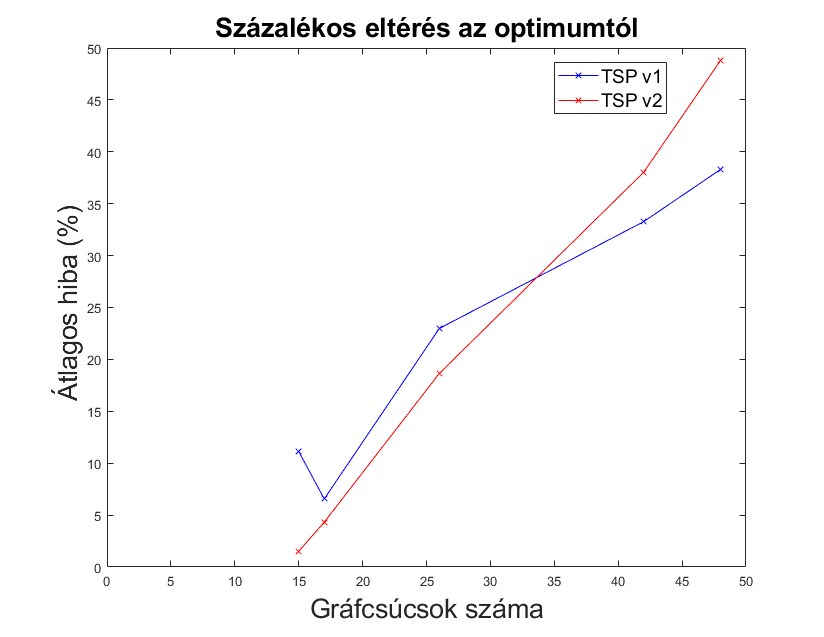
\includegraphics[width=75mm, keepaspectratio]{figures/TSP-benchmark-error.png}
	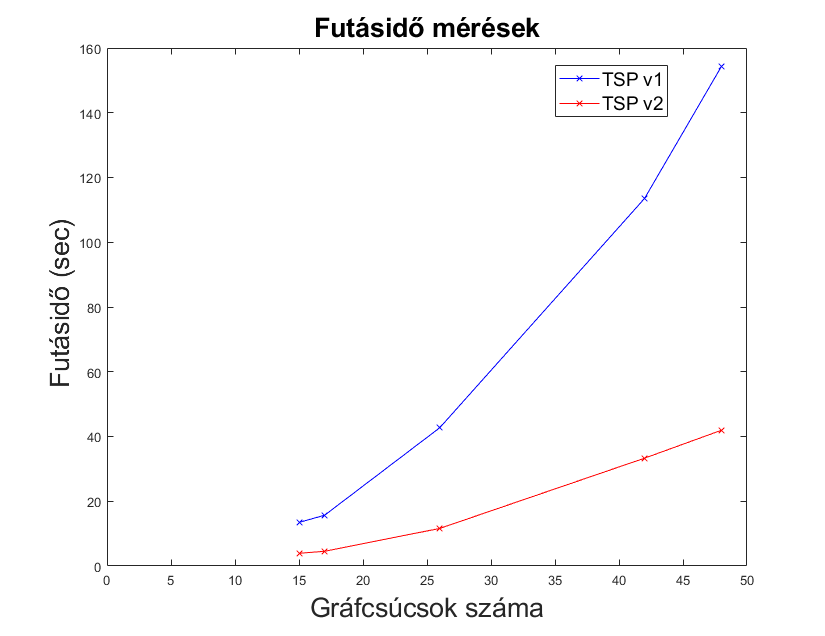
\includegraphics[width=75mm, keepaspectratio]{figures/TSP-benchmark-time.png}
	\caption{A két TSP verziót ugyanazon tesztadatokon futtattam. 20480 thread és 10 iteráció mellett Matlabban ábrázoltam a kapott eredményeket. Látható, hogy a TSP v2 hasonló eredmények mellett 3-4x gyorsabb futásra volt képes}
	\label{fig:TSP-benchmark}
\end{figure}

Mindkét implementációról elmondható, hogy nagyságrendekkel legyőzte a "Brute force" megoldást. Míg nyers összehasonlításokkal egy 48 csúcsú gráf összes lehetséges csúcssorrendjének kiértékelése évmilliókba telt volna, az ACO második verziója 30 iterációval képes volt erre 2 perc alatt úgy, hogy az optimális megoldástól átlagosan mindössze 41,2\%-kal hosszabb utat talált, legjobb esetben csak 31,6\%-kal. 10 iteráció esetében pedig mintegy 40 másodperc alatt átlagosan 48,8\%-kal múlta felül az optimális esetet.
  

\section{CVRP}
A kapacitásos járműútvonal-tervezési probléma méréseit a \ref{fig:CVRP-benchmark}. ábrán jelenítettem meg.

\begin{figure}[ht!]
	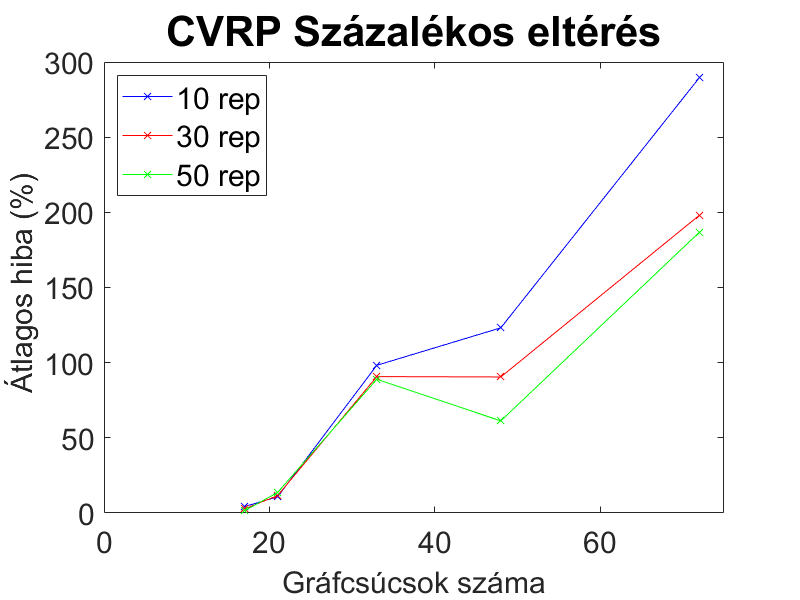
\includegraphics[width=75mm, keepaspectratio]{figures/CVRP-benchmark-error.png}
	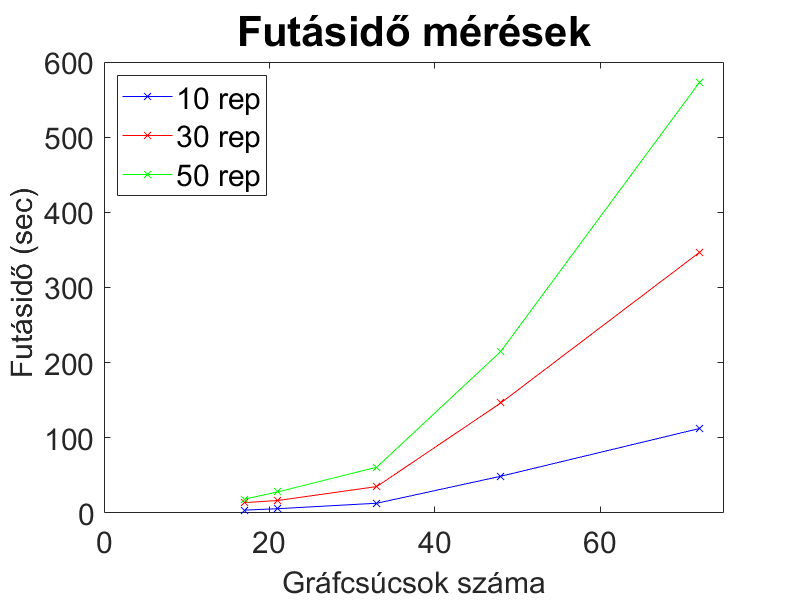
\includegraphics[width=75mm, keepaspectratio]{figures/CVRP-benchmark-time.png}
	\caption{A CVRP méréseket 20480 thread mellett ábrázoltam 10, 30 és 50 iteráció esetén}
	\label{fig:CVRP-benchmark}
\end{figure}

A grafikonról leolvasható az az elvárt jelenség, hogy hosszabb ideig futtatva a programot, több sorrendet megvizsgálva jobb lesz a végeredmény. Szubjektív megítélésem alapján jelen tesztadatokra érdemesebb 30 iteráció után megállni, mert az utolsó 20 vizsgálati sorozat viszonylag kis mértékben tudta csak javítani az outputot. 

\section{CVRPTW}
Az időablakokkal nehezített kapacitásos járműútvonal-tervezési probléma méréseit a \ref{fig:CVRPTW-benchmark}. ábrán jelenítettem meg, számtani közepeket képeztem a C201 és C202 mérésekből.

\begin{figure}[ht!]
	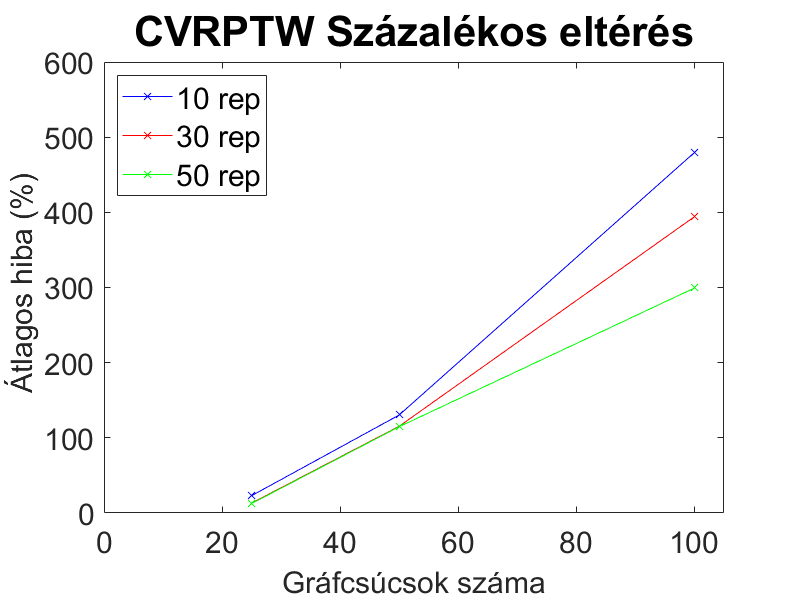
\includegraphics[width=75mm, keepaspectratio]{figures/CVRPTW-benchmark-error.png}
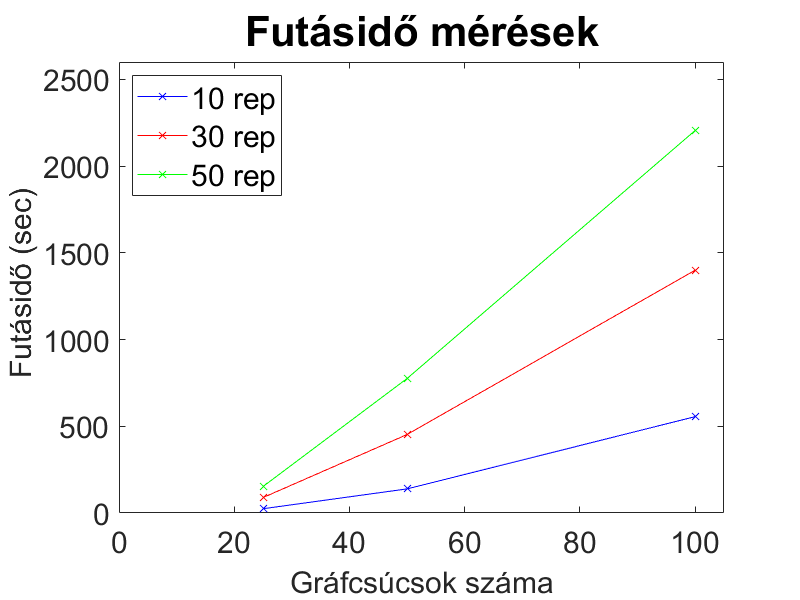
\includegraphics[width=75mm, keepaspectratio]{figures/CVRPTW-benchmark-time.png}
\caption{A CVRPTW méréseket 20480 thread mellett ábrázoltam 10, 30 és 50 iteráció esetén}
\label{fig:CVRPTW-benchmark}
\end{figure}

Az előzőkkel hasonlóan most is megemlíthető, hogy hosszabb ideig futtatva a programot jobb megoldást kapunk. Jelen esetben viszont ez olyan csekély javulásnak bizonyult, hogy esetleg érdemes lehet megállni 10 iteráció után. Egyedül a 100 csúcsú méréseknél volt észrevehető javulás: ott az 5-ször annyi várakozás eredményeképpen a végeredmény ~30\%-ot javult.

\section{Az összes probléma összevetése} \label{sec:allVRPresults}
Végül szeretném összehasonlítani, hogy mire jutottam a különböző problémák megoldása terén. Az első TSP verzióval most már nem foglalkozom, az ugyanis sohasem volt végterméknek szánva. Egységesen 20480 thread (20 teljes blokk) és 30 iteráció paraméterekkel a \ref{fig:allVRP-benchmark}. ábrán látható az összes algoritmus egymás mellett.

\begin{figure}[ht!]
	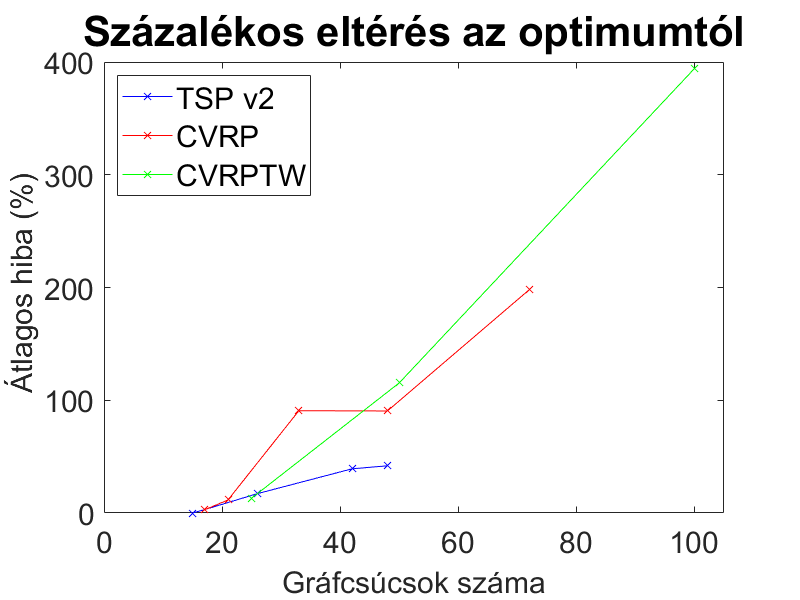
\includegraphics[width=75mm, keepaspectratio]{figures/allVRP-benchmark-error.png}
	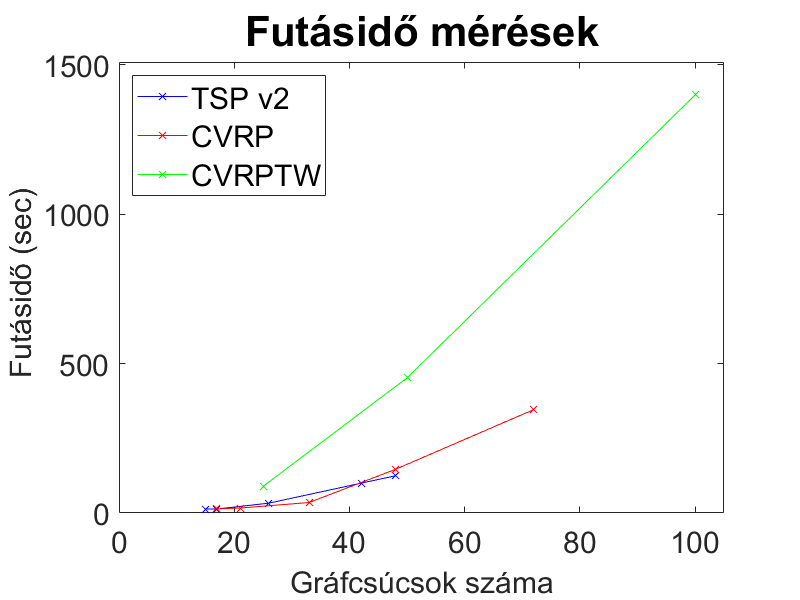
\includegraphics[width=75mm, keepaspectratio]{figures/allVRP-benchmark-time.png}
	\caption{20480 thread és 30 iteráció mellett megjelenítettem az egyes algoritmusok mérési eredményeit}
	\label{fig:allVRP-benchmark}
\end{figure}

Több dolog egyből látszik az ábrán. Az első észrevételem, hogy futásidőben \textbf{az összes mérés alacsony fokú polinomfüggvényekre hasonlít}, de természetesen ehhez nagyobb csúcsszámú mérések is kellenének. 

Második, hogy bár a többihez képest igencsak alacsony csúcsszám mellett próbáltam csak ki a TSP-t (nem találtam nagyobb adathalmazt), meglepően jól teljesített mind végeredmény, illetve futásidő tekintetében. Azért örvendetes hír ez a számomra, hiszen a gyakorlatban az Utazóügynök probléma merülhet fel a leggyakrabban. Egy SMD beültetőgép esetében például egy szerelőlemezt általában egy beültetőfej szokott kezelni.

Elemezzük a CVRP-t. Futásidő tekintetében elmondható, hogy tartotta az ütemet a TSP-vel kapcsolatban. Ez kifejezetten meglepett, hiszen egy n csúcsú, k járművel bejárt CVRP-t egy n+k-1 csúcsú TSP-re vezettem vissza. A végeredmény sokat romlott. Ezt annak a rovására írom, hogy jelentősen szűkült már közepes csúcsszám mellett is az érvényes megoldások halmaza.

Végül elemezzük a CVRPTW-t. Itt az előzőekhez képest a futásidő drasztikusan, mintegy 2-3-szorosára nőtt. Ennek a következők lehetnek az okai:
\begin{itemize}
	\item 1 iteráción belül CVRPTW esetén 200 random hangya generációt futtattam, míg korábban csak 20-at
	\item ha egy hangya nem volt sikeres, de csak az időablaok feltételét sértette meg, először rendeztem a bejárási tömbjét, majd újrasétáltattam
\end{itemize}
Elmondható tehát, hogy jelentősen romlott a sebességünk, de nyertünk vele egy nagyon fontos dolgot: a százalékos hiba terén sikerült elérni, hogy a CVRPTW hibagörbéje többé-kevésbé illeszkedjen a CVRP vonulatára. Magyarul: sikerült bizonyos mértékig kiküszöbölni az időzítés okozta nehézségeket.

\section{Összefoglalás}
Dolgozatom elkészültéhez közel másfél évi munkám volt szükséges, ezalatt részletesen megismerkedtem a párhuzamos programozás sajátos világával a CUDA keretrendszeren keresztül. Kezdetben olyan mátrixműveletek, mint a determinánsszámítás többszálú megvalósítása által tapasztaltam meg a GPU-ra történő memóriaátvitel, a szálkezelés, szinkronizálás, meg még sok egyéb okozta nehézségeket. Amikor már kicsit jobban értettem a CUDA használatához, belevágtam a genetikus algoritmusok témakörébe, és elkezdtem leprogramozni az Utazóügynök probléma első verzióját. Az Önálló laboratórium végére lettem vele készen. A szakdolgozat-készítés során javítottam az előző implementáción, valamint melléírtam a kapacitás-, illetve időablak-feltételeket előíró programjaimat. A végtermékek kapcsán úgy gondolom, hogy még sok mindent lehetne fejleszteni rajtuk (mindig lehet mindenen javítani), de elértek egy olyan szintre, hogy tényleg gyakorlatban bevethetőek legyenek. Munkámmal bizonyítottam, hogy a videokártyáknak igenis van helyük ilyen komoly számításigényű területen, mint a járművek feltételes útvonaltervezésének problémaköre.

\section{Továbbfejlesztési lehetőségek}

Munkám több módon is folytatható lenne. Amit mindig sajnáltam, hogy programjaim megmaradtak konzolos alkalmazásoknak. Lehetne a projektekhez implementálni akár egy egyszerű grafikus alkalmazást, ahol akár egyedi pontokat is fel lehetne venni a gráfba, és futás után a program vonalakkal szemléltetné a megtalált útvonalat. Van egy sokkal technikaibb észrevételem is: amikor egy tudatos hangya követi a feromonokat, mindig az összes csúcs közül sorsol magának. Ilyenkor ha már bejárt csúcsot választ, újrasorsoltatom, hiszen nem jó megoldás kétszer bejárni egy pontot. Ha eleve egy tömbben eltárolná mindegyik egyed, hogy merre járt már, a kiválasztási folyamat sokat egyszerűsödne, ami a futásidők jelentős rövidülését vonhatná magával.

\section{Kritériumfeltételek problémája a Hangyakolónia algoritmussal}
\label{section:conditionsWithACO}
Ahogy már korábban a \ref{sssec:HeldKarpEvaluate}. részben utaltam rá, a Hangyakolónia algoritmus számára is kihívással jár az, hogy ha a keresett útvonal különböző feltételeknek maradéktalanul meg kell feleljen. Dolgozatomban kétféle feltételrendszert vizsgáltam: a járművek korlátozott kapacitását, illetve a felhasználók megszabott időbeosztását. A CVRP esetében Most összefoglalnám, hogy miért érhettek el a feltételes esetben végzett méréseim jelentősen rosszabb eredményeket.

Az ACO úgy működik, hogy eleinte a gyengébb megoldásokból generál egyre jobbakat. Feltételezi, hogy találunk megoldást, amit javítani tudunk. A kritériumfeltételek olyanok, hogy vagy teljesülnek, vagy nem. Nehéz úgy értékelni, hogy az első csak kicsit hibázott, a következő közepesen stb. Ha rossz, akkor nem engedhetjük a megoldáshalmazba.

Most azt nézném meg, hogy ha véletlenszerű csúcssorrendeket generálok úgy, ahogyan ezt a hangyák is teszik az ACO-ban, akkor mekkora annak a valószínűsége, hogy találunk egy, a kritériumnak megfelelő megoldást.

Ha egy esemény bekövetkezési valószínűsége p, akkor annak a valószínűsége, hogy n-szer ismételve az eseményt legalább 1 alkalommal bekövetkezik, binomiális valószínűségi eloszlás szerint:
\begin{equation}
	P(x>0) = 1-(1-p)^n
	\label{binomial_probability}
\end{equation}

\subsection{Kapacitásfeltétel}
Kezdjük a kapacitáskritériummal, mert az az egyszerűbb. Az első 5 adathalmazban minden csúcs igénye 1, vagyis azt kell néztünk, hogy az egyes járművek hány csúcsot járnak be. A kezdőcsúcsot nem kell beleszámolni, mert annak nincs igénye. 

Probléma: Az (n-1) db csúcsot véletlenszerűen szétosztjuk k db jármű között. Mennyi annak a valószínűsége, hogy egyik járműhöz sem osztanak több, mint C db-ot? Első példa (gr17): 16 állomás, 3 jármű, a járművek kapacitása 6. \(p_{gr17}=?\)

\newcommand{\pgr}{0,258}

Csak 6-6-4 vagy 6-5-5 felosztásban lehetnek a csúcsok. Az összes eset \(3^{16}\), mert minden csúcsra eldöntjük, hogy melyik járműhöz osztjuk be. Összesen \(\binom{16}{6}*\binom{10}{6}*3 + \binom{16}{6}*\binom{10}{5}*3 \) esetben nem lesz több, mint 6 egyik jármű kapacitása sem.
\begin{equation}
	p_{gr17} = 3*\frac{\binom{16}{6}*\binom{10}{6} + \binom{16}{6}*\binom{10}{5}}{3^{16}} \approx \pgr
	\label{gr17_p}
\end{equation}
Nézzük meg az att48-ra is ugyanezt: \((n-1)=47\) állomás, k=3 jármű, a járművek kapacitása C=16. \(p_{att48}=?\)

\newcommand{\patt}{0,051}

Ebben a problémában csak 16-16-15 felosztásban lehetnek a csúcsok. Az előbbi példához hasonlóan gondolkozva a valószínűség:

\begin{equation}
	p_{gr17} = \frac{3*\binom{47}{16}*\binom{31}{16}}{3^{47}} \approx \patt
	\label{att48_p}
\end{equation}

\newcommand{\nInTenIterations}{4096000}

Ha 20480 szálon 10 iterációt végzek, és 1 iteráción belül 20-szor generálok egymás után random sorrendet, akkor összesen n=\nInTenIterations kísérletet végzek. A \ref{binomial_probability}. egyenletbe behelyettesítve annak a valószínűsége, hogy találok megoldást:

\begin{equation}
	P_{gr17} = 1-(1-\pgr)^{\nInTenIterations} = 1
	\label{gr17_P}
\end{equation}

\begin{equation}
	P_{att48} = 1-(1-\patt)^{\nInTenIterations} = 1
	\label{att48_P}
\end{equation}

Ezek alapján nem meglepő, hogy mindig találtam megoldást a CVRP tesztelése során.

\subsection{Időablakok feltétele}
Most jön annak a vizsgálata, hogy miért nem találtam megoldást olyan sok esetben a CVRPTW mérésekor. Sajnos itt már nem lehet olyan szépen intuitívan megállapítani egy adott problémában egy véletlenszerű bejárás megfelelőségének a valószínűségét. 